\documentclass[10pt,a4paper]{article}

\usepackage{fontspec}
\defaultfontfeatures{Ligatures=TeX}
\setmainfont{DejaVu Serif}
\setsansfont{DejaVu Sans}
\setmonofont{DejaVu Sans Mono}[Scale=0.86]

\usepackage[a4paper,top=2.35cm,bottom=2.35cm,left=2.35cm,right=2.35cm,headheight=13pt]{geometry}
\usepackage{microtype}
\usepackage{setspace}
\usepackage{graphicx}
\usepackage{booktabs}
\usepackage{tabularx}
\usepackage{array}
\usepackage{multirow}
\usepackage{float}
\usepackage{enumitem}
\usepackage{tikz}
\usepackage{xcolor}
\usepackage{hyperref}
\usepackage{caption}
\usepackage{amsmath}
\usepackage{titlesec}
\usepackage{fancyhdr}

\usetikzlibrary{arrows.meta,positioning,shapes.geometric}
\graphicspath{{figures/}}

\hypersetup{
    colorlinks=true,
    linkcolor=black,
    urlcolor=black,
    citecolor=black
}

\setstretch{1.04}
\setlength{\parindent}{1.2em}
\setlength{\parskip}{0pt}
\setlength{\abovedisplayskip}{5pt plus 2pt minus 2pt}
\setlength{\belowdisplayskip}{5pt plus 2pt minus 2pt}
\setlength{\textfloatsep}{8pt plus 2pt minus 2pt}
\setlength{\floatsep}{7pt plus 2pt minus 2pt}
\setlength{\intextsep}{7pt plus 2pt minus 2pt}
\setlist[itemize]{topsep=2pt,itemsep=1pt,parsep=0pt,leftmargin=1.35em}
\setlist[enumerate]{topsep=2pt,itemsep=1pt,parsep=0pt,leftmargin=1.45em}
\renewcommand{\arraystretch}{1.12}
\captionsetup{font=small,labelfont=bf,labelsep=period}
\titlespacing*{\section}{0pt}{13pt plus 2pt minus 2pt}{5pt}
\titlespacing*{\subsection}{0pt}{9pt plus 2pt minus 2pt}{4pt}
\titleformat{\section}{\large\bfseries}{\thesection}{0.7em}{}
\titleformat{\subsection}{\normalsize\bfseries}{\thesubsection}{0.7em}{}
\fancyhf{}
\fancyhead[L]{\footnotesize\itshape\nouppercase{\leftmark}}
\fancyfoot[C]{\footnotesize\thepage}
\renewcommand{\headrulewidth}{0.35pt}
\renewcommand{\footrulewidth}{0pt}
\emergencystretch=2em

\newcolumntype{Y}{>{\raggedright\arraybackslash}X}
\newcommand{\code}[1]{\texttt{#1}}

\title{Dự đoán xu hướng giá dầu ngày kế tiếp bằng Data Mining và Machine Learning}
\author{}
\date{2026}

\begin{document}
\pagestyle{plain}

% =========================
% Cover page
% =========================
\begin{titlepage}
    \centering
    \thispagestyle{empty}
    \vspace*{0.9cm}
    {\large \textbf{BÁO CÁO MÔN HỌC}}\\[0.25cm]
{\normalsize CS313}\\[1.25cm]

    {\LARGE \textbf{Dự đoán xu hướng giá dầu ngày kế tiếp}}\\[0.25cm]
    {\large bằng Data Mining và Machine Learning}\\[1.05cm]

    {\small
    \begin{tabular}{rl}
        \textbf{Bài toán:} & Phân loại nhị phân UP/DOWN cho giá dầu ngày kế tiếp \\
        \textbf{Dữ liệu:} & Bộ dữ liệu đã xử lý và kiểm soát leakage \\
        \textbf{Số dòng:} & 2,922 quan sát theo ngày \\
        \textbf{Số feature:} & 27 feature sau xử lý và kiểm soát leakage \\
        \textbf{Thời gian test:} & target date từ 2023-01-01 trở đi \\
    \end{tabular}
    }

    \vfill

    \textbf{Danh sách thành viên nhóm:}\\[0.35cm]

    {\small
    \renewcommand{\arraystretch}{1.22}
    \begin{tabular}{|c|l|l|l|}
    \hline
    \textbf{STT} & \textbf{Tên sinh viên} & \textbf{MSSV} & \textbf{Nhiệm vụ} \\
    \hline
    1 & Phan Thị Xuân Tiên & 23521584 & \\
    \hline
    2 & Đặng Quốc Thịnh & 23521494 & \\
    \hline
    3 & Lê Khắc Thuận & 23521550 & \\
    \hline
    4 & Nguyễn Minh Triết & 23521652 & \\
    \hline
    5 & Nguyễn Trần Nhật Trung & 23521684 & \\
    \hline
    \end{tabular}
    }

    \vspace{0.75cm}

    \textbf{Lớp:} CS313.Q23\\[0.55cm]
    \textbf{Giảng viên hướng dẫn:} TS. Võ Nguyễn Lê Duy

    \vspace*{0.7cm}
\end{titlepage}

% =========================
% TOC page
% =========================
\pagenumbering{roman}
\tableofcontents
\clearpage
\pagenumbering{arabic}
\pagestyle{fancy}

% =========================
% Content
% =========================
\section{Tóm tắt và xác định bài toán}

Báo cáo này trình bày pipeline Data Mining và Machine Learning cho bài toán dự đoán xu hướng giá dầu thô ngày kế tiếp. Nhãn được định nghĩa là:

\[
y_t =
\begin{cases}
1, & \text{nếu } oil\_return\_fwd1 > 0 \\
0, & \text{ngược lại}
\end{cases}
\]

Đây là bài toán \textbf{predictive data mining}, cụ thể là \textbf{supervised binary time-series classification} \cite{han2012,hastie2009}. Dữ liệu gồm các quan sát theo ngày; mỗi dòng có feature thị trường, vĩ mô, cung/cầu, tin tức/sentiment và geopolitical; đầu ra là nhãn UP/DOWN cho ngày kế tiếp. Vì target nằm ở tương lai, pipeline phải chia dữ liệu theo thời gian và tránh dùng thông tin nhìn trước.

Lý do chọn bài toán này là giá dầu thô có ý nghĩa kinh tế thực tế và đang chịu ảnh hưởng mạnh từ xung đột Trung Đông, rủi ro eo Hormuz, chiến sự Nga--Ukraine, sanctions và thay đổi trade flows. Trong bối cảnh giá dầu quanh vùng cao và biến động mạnh, dự đoán hướng giá ngày kế tiếp là bài toán khó nhưng phù hợp với Data Mining: khai phá xem dữ liệu đa nguồn có tạo được tín hiệu dự báo ngoài chuỗi giá đơn thuần hay không.

Kết quả tốt nhất trên strict final test là ensemble \code{ENS\_FINAL3}, đạt \textbf{Accuracy = 0.5476}, \textbf{F1-macro = 0.5406}, và \textbf{AUC = 0.5351}. Đây không phải kết quả rất mạnh, nhưng là baseline hợp lý cho daily next-day oil direction vì tín hiệu yếu, nhiễu lớn, và đánh giá được thực hiện theo thời gian.

\section{Dữ liệu, EDA và xử lý feature}

\subsection{Nguyên lý Data Mining áp dụng}

Pipeline phân tích bám theo quy trình KDD/CRISP-DM: xác định mục tiêu, hiểu dữ liệu, chuẩn bị dữ liệu, khai phá bằng mô hình, đánh giá và diễn giải kết quả \cite{fayyad1996,shearer2000}. Trong bài này, ``data mining'' không chỉ là bước train model, mà là toàn bộ quá trình biến dữ liệu thô từ nhiều nguồn thành tri thức có thể kiểm chứng: liệu dữ liệu thị trường, vĩ mô, cung/cầu, tin tức và xung đột có dự đoán được hướng giá dầu ngày kế tiếp hay không.

\begin{table}[!htbp]
\centering
\caption{Mapping giữa nguyên lý Data Mining và pipeline phân tích}
\small
\begin{tabularx}{0.98\linewidth}{lY}
\toprule
\textbf{Bước Data Mining} & \textbf{Cách thực hiện} \\
\midrule
Data selection & Chọn các nguồn liên quan đến giá dầu: market, FRED, EIA, GDELT và ACLED. \\
Data understanding & Kiểm tra phạm vi thời gian, missing values, kiểu dữ liệu, duplicate và thống kê mô tả. \\
Data cleaning & Xử lý missing, chuẩn hóa ngày, gộp sự kiện cuối tuần về ngày giao dịch kế tiếp và forward-fill có giới hạn. \\
Data integration & Gộp nhiều nguồn vào cùng business-day timeline và kiểm tra trùng lặp hoặc redundancy. \\
Transformation/reduction & Tạo return, lag, rolling window, log/signed-log, scale và loại các cột có nguy cơ leakage. \\
Mining/modeling & So sánh baseline, feature selection, weight decay, ensemble và deep learning để khai phá tín hiệu dự đoán. \\
Evaluation/interpretation & Dùng chronological validation/test, F1-macro, Accuracy, AUC, MCC và confusion matrix để diễn giải model thay vì chỉ nhìn một con số accuracy. \\
\bottomrule
\end{tabularx}
\end{table}

\subsection{Nguồn dữ liệu, thu thập và quyền truy cập}

Các nguồn dữ liệu được lấy theo hai cách: API chính thức có API key, hoặc file public/manual export. Với báo cáo môn học, nhóm chỉ dùng dữ liệu cho mục đích học thuật và trình bày kết quả tổng hợp; không nên công khai lại raw data hoặc API key.

\begin{table}[!htbp]
\centering
\caption{Nguồn dữ liệu, phương thức thu thập và yêu cầu truy cập}
\scriptsize
\begin{tabularx}{\linewidth}{lY Y}
\toprule
\textbf{Nguồn} & \textbf{Cách thu thập} & \textbf{Quyền truy cập / lưu ý sử dụng} \\
\midrule
Yahoo Finance & Lấy dữ liệu thị trường như Brent oil, Dollar Index, S\&P500 và VIX thông qua thư viện hỗ trợ truy cập Yahoo Finance. & Đây là nguồn phù hợp cho research/education; không nên phát hành lại raw market data, chỉ trình bày kết quả tổng hợp hoặc feature đã xử lý \cite{yahooYfinance}. \\
FRED & Lấy các biến vĩ mô như lãi suất, CPI, thất nghiệp, yield spread và WTI thông qua API chính thức. & Cần FRED account và API key riêng. Khi dùng trong báo cáo cần ghi nguồn FRED/nguồn gốc series \cite{fredApi}. \\
EIA & Lấy dữ liệu tồn kho, sản lượng và net imports dầu thô thông qua API chính thức. & Cần đăng ký EIA API key. Dữ liệu public được cung cấp miễn phí, nhưng cần ghi nguồn U.S. Energy Information Administration và tuân thủ API Terms \cite{eiaApi}. \\
GDELT & Tải dữ liệu sự kiện public theo ngày, lọc các sự kiện liên quan Trung Đông rồi tổng hợp tone, Goldstein score và volume. & GDELT cung cấp event data public. Cần truy cập với tần suất hợp lý và ghi nguồn GDELT khi dùng dữ liệu \cite{gdeltData}. \\
ACLED & Export dữ liệu từ ACLED Data Export Tool, sau đó tổng hợp số sự kiện và fatalities theo ngày giao dịch. & Cần đăng ký ACLED Access Portal và đồng ý Terms/Attribution Policy. Không được chia sẻ lại raw ACLED data; báo cáo chỉ dùng feature tổng hợp \cite{acledTerms}. \\
\bottomrule
\end{tabularx}
\end{table}

\subsection{Dữ liệu và split}

Bộ dữ liệu cuối cùng gồm 2,922 dòng theo ngày và 27 feature sau xử lý. Tập test không được chọn ngẫu nhiên mà là giai đoạn tương lai từ 2023-01-01 trở đi. Cách chia này mô phỏng đúng tình huống thực tế: mô hình học từ quá khứ và dự đoán giai đoạn chưa thấy.

\begin{table}[!htbp]
\centering
\caption{Thiết kế train/validation/test theo thời gian}
\small
\begin{tabular}{lrrrr}
\toprule
\textbf{Split} & \textbf{Điều kiện target date} & \textbf{Số dòng} & \textbf{UP rate} & \textbf{Std return} \\
\midrule
Train & $< 2022$ & 1,822 & 0.5143 & 0.0259 \\
Validation & 2022 & 260 & 0.5077 & 0.0286 \\
Train full & $< 2023$ & 2,082 & 0.5134 & 0.0263 \\
Test & $\geq 2023$ & 840 & 0.4976 & 0.0195 \\
\bottomrule
\end{tabular}
\end{table}

\noindent{\footnotesize \code{Train full} không phải là một holdout split độc lập. Nó chính là toàn bộ dữ liệu trước năm 2023, tức \code{Train + Validation}. Model được train lần đầu trên \code{Train} để chọn threshold/hyperparameter bằng \code{Validation}; sau khi các lựa chọn đã khóa, model cuối được refit trên \code{Train full} rồi mới dự đoán \code{Test}. Tập \code{Test} không tham gia train, chọn feature hay chọn threshold.}

\begin{figure}[!htbp]
\centering
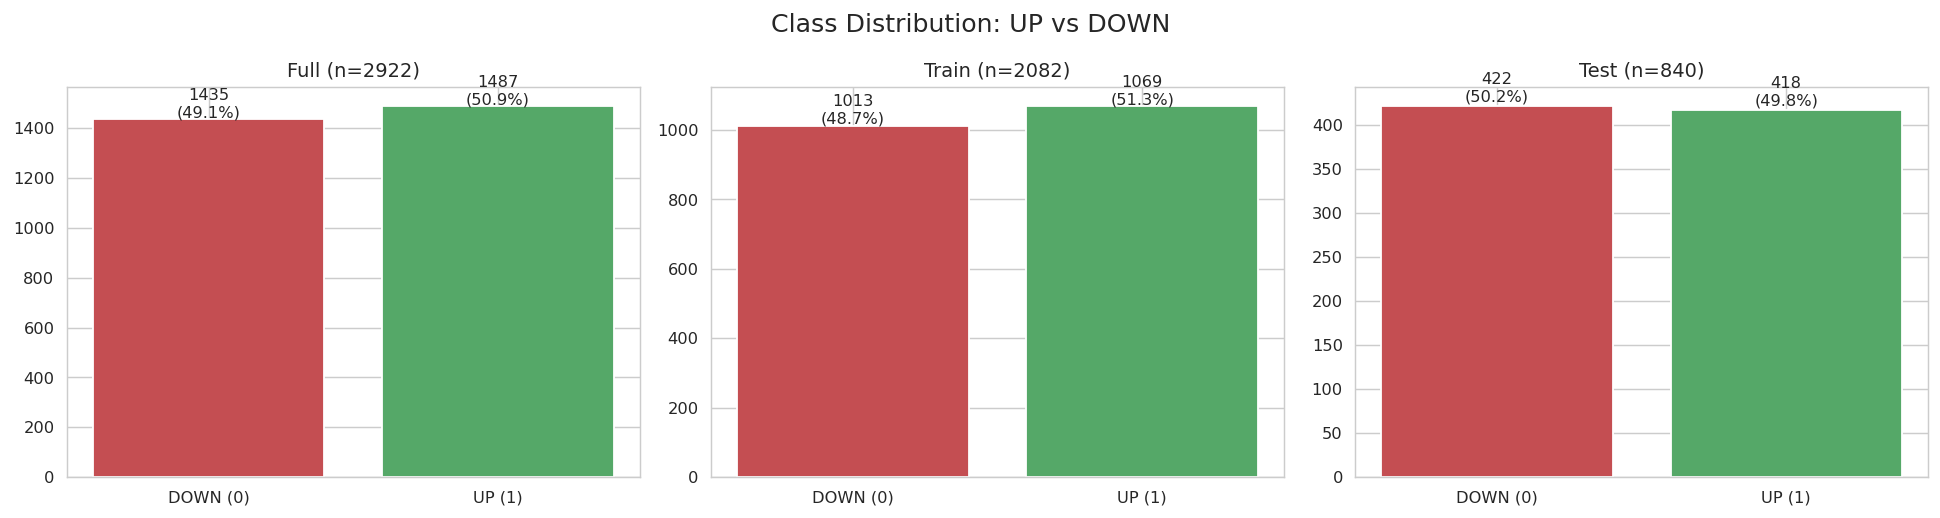
\includegraphics[width=0.92\linewidth]{class_distribution.png}
\caption{Phân bố nhãn UP/DOWN sau khi chia train/test theo thời gian}
\end{figure}

EDA cho thấy nhãn khá cân bằng: train có UP khoảng 51.3\%, test có UP khoảng 49.8\%. Vì vậy, bài toán không thể được giải thích bằng cách đoán một lớp. Tuy nhiên, các feature chỉ có tín hiệu yếu: 10/27 feature có KS test đáng kể, 11/27 feature có Mann-Whitney đáng kể, 7/27 feature có point-biserial đáng kể, và không có feature nào có Cohen's $d > 0.2$. Điều này giải thích vì sao mô hình chỉ đạt edge nhỏ thay vì accuracy rất cao.

\subsection{Feature và xử lý dữ liệu}

Các feature được giữ gọn để giảm leakage và giảm nhiễu. Nhóm feature chính được tóm tắt trong Bảng~\ref{tab:feature-groups}. Phần xử lý tập trung vào ba mục tiêu: tạo target forward return đúng thời điểm, loại feature có nguy cơ dùng thông tin tương lai, và biến đổi/scale các biến lệch phân phối.

\begin{table}[!htbp]
\centering
\caption{Nhóm feature chính sau xử lý}
\label{tab:feature-groups}
\small
\begin{tabularx}{0.98\linewidth}{lY}
\toprule
\textbf{Nhóm} & \textbf{Feature tiêu biểu và vai trò} \\
\midrule
Market/return & \code{oil\_return}, \code{oil\_return\_lag1}, \code{oil\_return\_lag2}, \code{usd\_return}, \code{sp500\_return}, \code{vix\_return\_slog1p}; mô tả trạng thái thị trường và rủi ro. \\
Macro/rate & \code{yield\_spread}; phản ánh môi trường lãi suất và kỳ vọng kinh tế. \\
Supply/inventory & \code{inventory\_change\_pct}, \code{inventory\_zscore}, \code{net\_imports\_change\_pct\_slog1p}, \code{production\_change\_pct\_slog1p}; mô tả cung/cầu dầu. \\
News/sentiment & \code{gdelt\_goldstein}, \code{gdelt\_tone\_7d}, \code{gdelt\_tone\_30d}, \code{gdelt\_volume\_lag1\_log1p}; khai thác tín hiệu tin tức. \\
Geopolitical & \code{conflict\_event\_count\_log1p}, \code{conflict\_intensity\_7d\_log1p}, \code{fatalities\_log1p}; mô tả rủi ro địa chính trị. \\
Calendar & \code{day\_of\_week\_sin/cos}, \code{month\_sin/cos}; mã hóa chu kỳ ngày trong tuần và tháng. \\
\bottomrule
\end{tabularx}
\end{table}

\begin{figure}[!htbp]
\centering
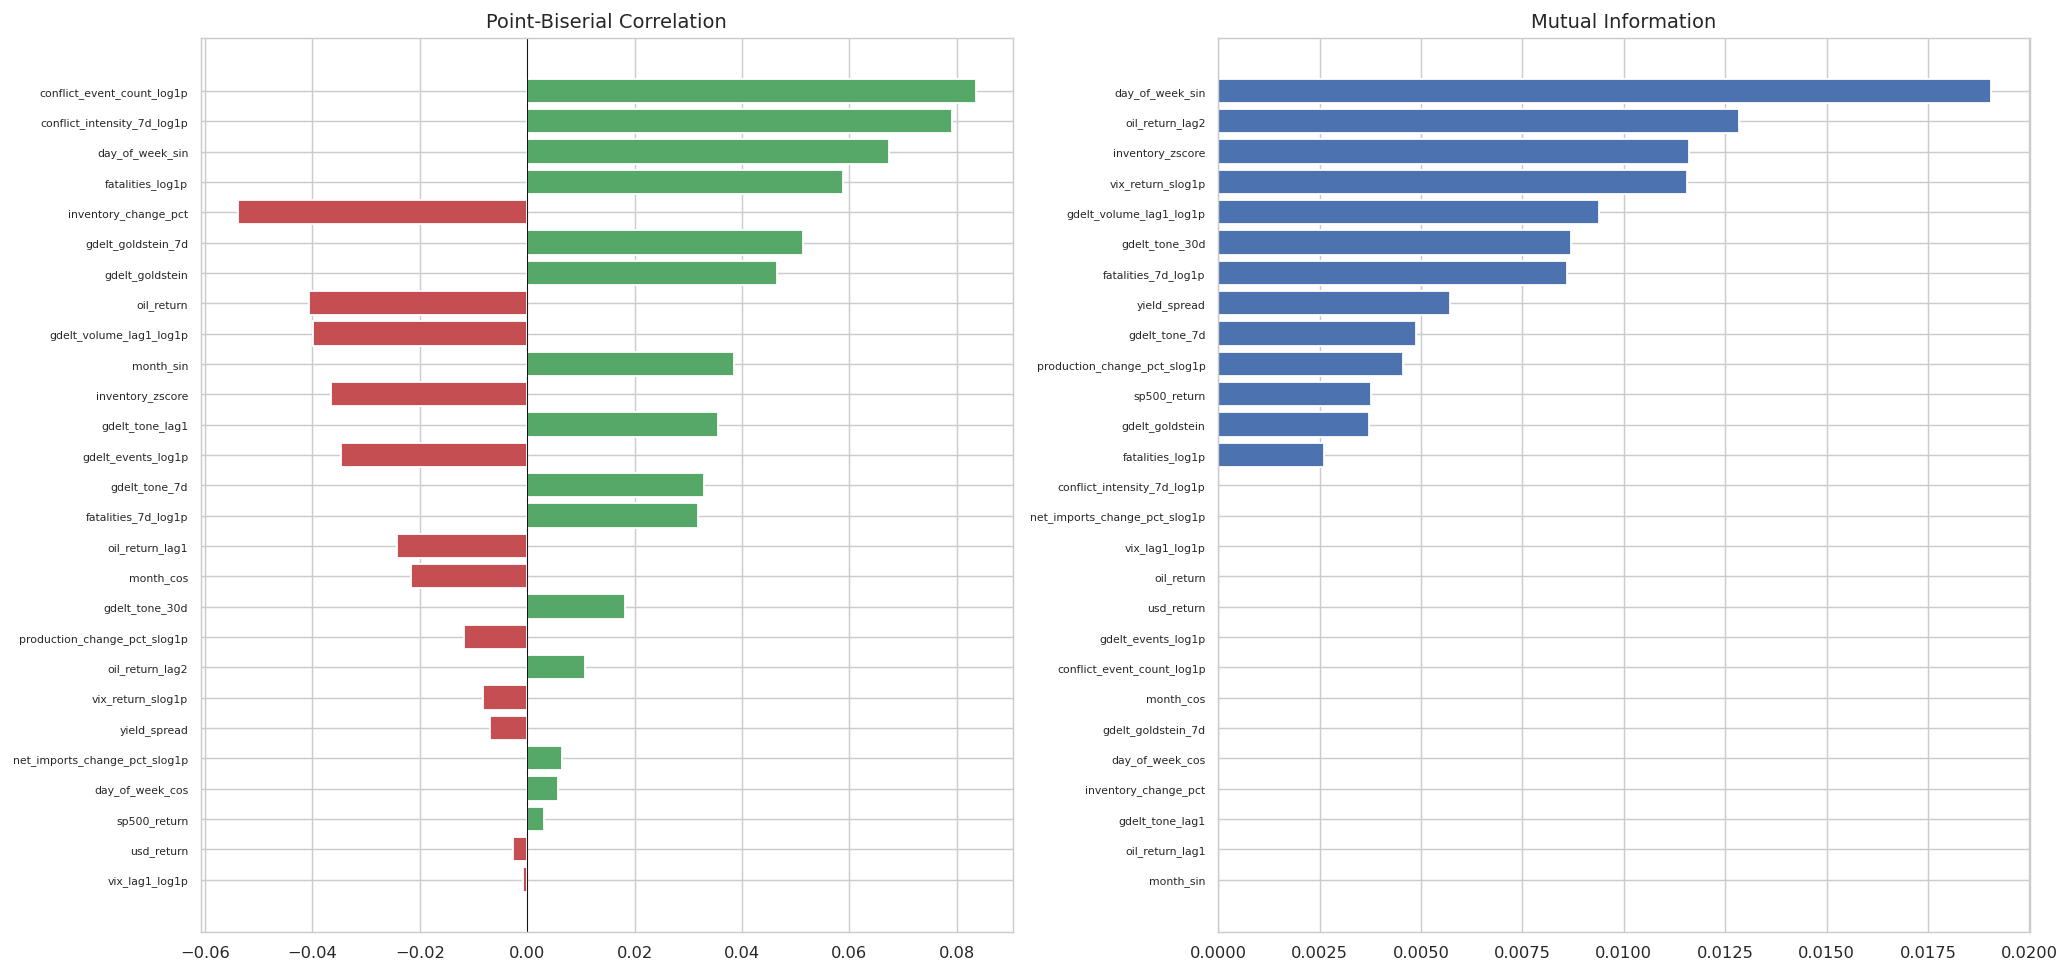
\includegraphics[width=0.86\linewidth]{feature_signal_scores.png}
\caption{Tín hiệu feature theo EDA: feature có ích nhất vẫn chỉ tạo phân tách yếu giữa hai lớp}
\end{figure}

Về data mining, EDA và xử lý feature là bước khai phá xem dữ liệu có chứa pattern dự đoán hay không. Các feature như \code{day\_of\_week\_sin}, \code{gdelt\_goldstein}, \code{gdelt\_tone\_7d}, \code{inventory\_zscore}, \code{conflict\_event\_count\_log1p} có ranking tốt hơn các feature khác, nhưng mức phân tách vẫn nhỏ. Vì vậy, chiến lược phù hợp là đánh giá nhiều họ mô hình trong cùng một setup, thay vì kỳ vọng một model đơn lẻ tạo ra bước nhảy lớn.

\section{Thiết kế mô hình và đánh giá}

Pipeline so sánh 33 cấu hình cuối cùng, gồm baseline, feature selection, weight decay, ensemble và deep learning. Tất cả model dùng cùng target, cùng split theo thời gian, cùng strict final test và cùng threshold chính \code{fixed\_0.5}. Điều này giúp bảng kết quả có thể so sánh trực tiếp.

\begin{figure}[!htbp]
\centering
\begin{tikzpicture}[
    node distance=0.35cm,
    box/.style={rectangle, rounded corners, draw=black, align=center, minimum width=2.18cm, minimum height=0.62cm, font=\scriptsize},
    arrow/.style={-{Latex}, thick}
]
\node[box] (data) {Dữ liệu\\đã xử lý};
\node[box, right=of data] (split) {Chronological\\split};
\node[box, right=of split] (val) {Validation\\2022};
\node[box, right=of val] (refit) {Refit\\$<2023$};
\node[box, right=of refit] (test) {Strict test\\2023+};
\draw[arrow] (data) -- (split);
\draw[arrow] (split) -- (val);
\draw[arrow] (val) -- (refit);
\draw[arrow] (refit) -- (test);
\end{tikzpicture}
\caption{Luồng đánh giá theo thời gian để giảm nguy cơ leakage}
\end{figure}

\begin{table}[!htbp]
\centering
\caption{Các nhóm mô hình được đánh giá}
\small
\begin{tabularx}{0.98\linewidth}{lcY}
\toprule
\textbf{Nhóm} & \textbf{Số config} & \textbf{Câu hỏi kiểm tra} \\
\midrule
Baseline & 7 & Các classifier phổ biến có tìm được tín hiệu cơ bản không? \\
Feature selection & 4 & Giảm feature nhiễu có cải thiện kết quả không? \\
Weight decay & 10 & Ưu tiên dữ liệu gần hơn có giúp xử lý regime shift không? \\
Ensemble & 4 & Trung bình xác suất từ nhiều model yếu có ổn định hơn không? \\
Deep learning & 8 & Lookback sequence 5--40 ngày có thêm tín hiệu so với tabular ML không? \\
\bottomrule
\end{tabularx}
\end{table}

Trong nhánh feature selection, số lượng feature không được xem là quyết định cố định ở bước preprocessing. Sau xử lý dữ liệu, pipeline có 27 feature hợp lệ; các mức 8, 12, 16, 20, 25 và toàn bộ 27 feature được xem như các lựa chọn hyperparameter. Cách làm này phù hợp với hướng dẫn của Guyon và Elisseeff về feature selection \cite{guyon2003}, đồng thời tránh lỗi selection bias được Ambroise và McLachlan \cite{ambroise2002}, cũng như Cawley và Talbot \cite{cawley2010},  feature selection nằm trong vòng train/validation, không dùng test để chọn feature nên không bị leakage. Trong pipeline này, subset được chọn bằng cross-validation theo thời gian trên train split; kết quả là nhóm 25 feature theo Spearman.

F1-macro được dùng làm metric chính vì hai lớp UP và DOWN đều quan trọng. Accuracy cho biết tỷ lệ dự đoán đúng tổng thể, AUC đo khả năng xếp hạng xác suất, còn MCC và Balanced Accuracy giúp kiểm tra mô hình có thiên lệch quá mạnh về một lớp hay không.

\section{Phân tích kết quả model}

\subsection{Kết quả leaderboard}

Bảng~\ref{tab:top-models} trình bày các model tốt nhất trên strict final test. Kết quả quan trọng nhất là \code{ENS\_FINAL3}: model này không train thêm estimator mới, mà lấy trung bình xác suất từ ba model tabular tốt và tương đối ổn định: \code{LGBM\_exp100}, \code{GBM\_exp100}, và \code{XGB\_linear03} \cite{chen2016,ke2017}.

\begin{table}[!htbp]
\centering
\caption{Top model trên strict final test}
\label{tab:top-models}
\small
\begin{tabular}{llrrrrr}
\toprule
\textbf{Nhóm} & \textbf{Model} & \textbf{Acc.} & \textbf{F1} & \textbf{AUC} & \textbf{MCC} & \textbf{N} \\
\midrule
Ensemble & ENS\_FINAL3 & 0.5476 & 0.5406 & 0.5351 & 0.0970 & 840 \\
Weight decay & LGBM\_exp100 & 0.5345 & 0.5341 & 0.5234 & 0.0695 & 840 \\
Weight decay & GBM\_exp100 & 0.5262 & 0.5256 & 0.5103 & 0.0522 & 840 \\
Baseline & BASE\_MLP & 0.5238 & 0.5232 & 0.5369 & 0.0481 & 840 \\
Baseline & BASE\_LogReg & 0.5167 & 0.5142 & 0.5250 & 0.0330 & 840 \\
Deep learning & DL\_GRU\_L40 & 0.5167 & 0.5138 & 0.5362 & 0.0330 & 840 \\
\bottomrule
\end{tabular}
\end{table}

\begin{figure}[!htbp]
\centering
\begin{minipage}[t]{0.60\linewidth}
    \centering
    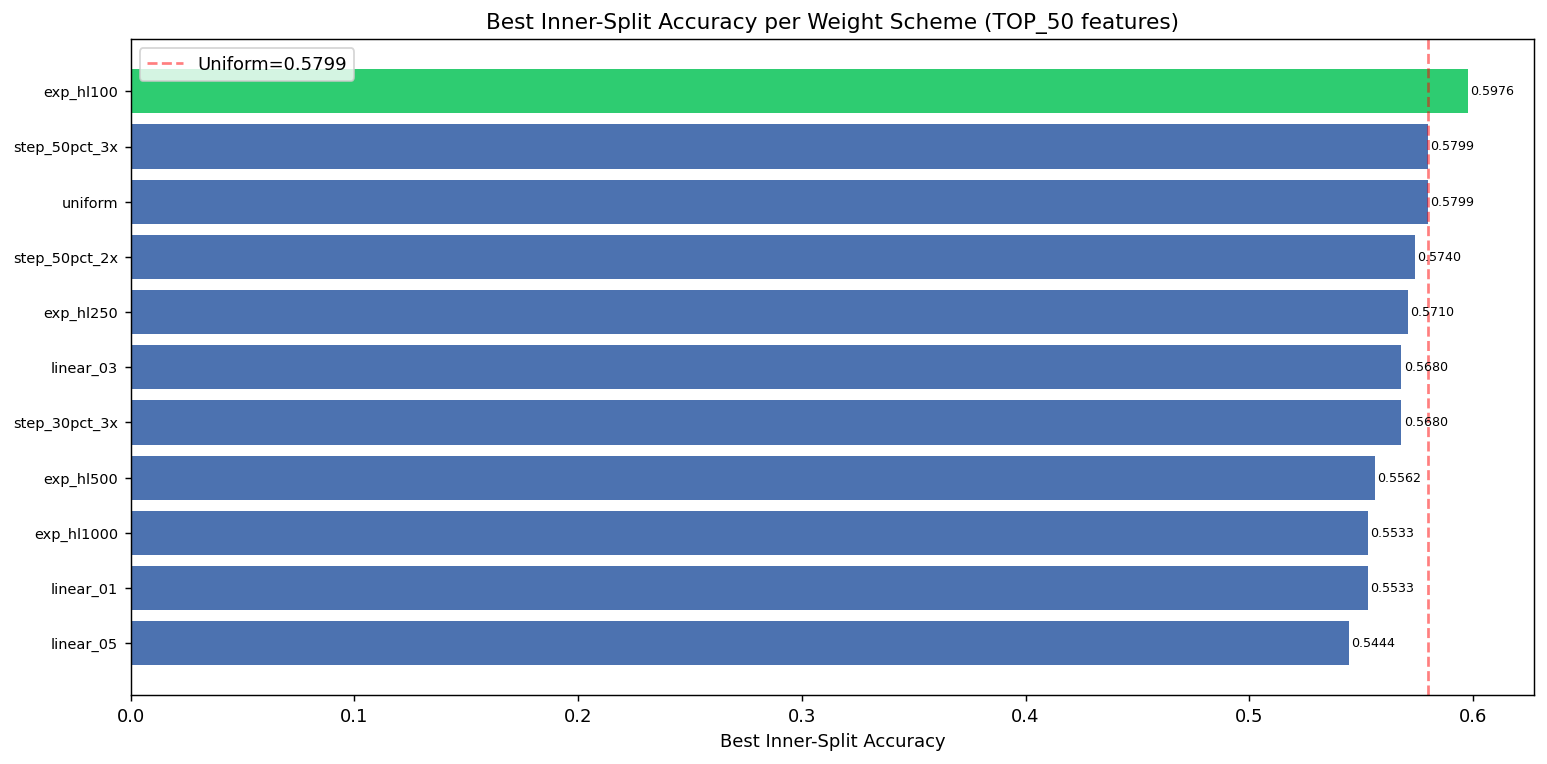
\includegraphics[width=\linewidth]{model_comparison.png}
    \caption{So sánh các nhóm model trong pipeline}
\end{minipage}
\hfill
\begin{minipage}[t]{0.34\linewidth}
    \centering
    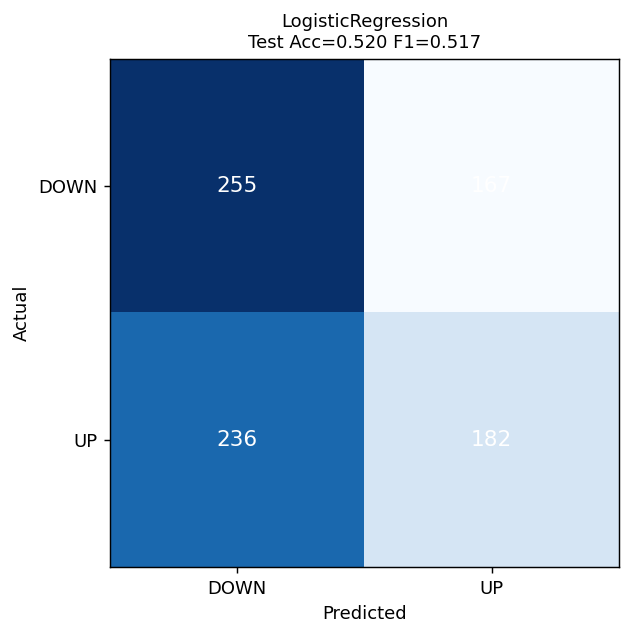
\includegraphics[width=\linewidth]{confusion_matrix.png}
    \caption{Confusion matrix từ nhánh classification}
\end{minipage}
\end{figure}

Điểm chính không phải là mô hình đạt accuracy cao, mà là pattern của toàn bộ bảng: phần lớn model nằm quanh 0.50--0.53, còn model tốt nhất chỉ lên 0.5476. Pattern này cho thấy bài toán có tín hiệu nhưng yếu. Nếu một mô hình đơn lẻ đạt 0.80--0.90 trong setup này thì cần ưu tiên kiểm tra leakage, random split, hoặc feature nhìn trước tương lai.

\subsection{So sánh theo nhóm phương pháp}

\begin{table}[!htbp]
\centering
\caption{Model tốt nhất trong từng nhóm}
\small
\begin{tabular}{llrrrr}
\toprule
\textbf{Nhóm} & \textbf{Best model} & \textbf{Acc.} & \textbf{F1} & \textbf{AUC} & \textbf{MCC} \\
\midrule
Ensemble & ENS\_FINAL3 & 0.5476 & 0.5406 & 0.5351 & 0.0970 \\
Weight decay & LGBM\_exp100 & 0.5345 & 0.5341 & 0.5234 & 0.0695 \\
Baseline & BASE\_MLP & 0.5238 & 0.5232 & 0.5369 & 0.0481 \\
Deep learning & DL\_GRU\_L40 & 0.5167 & 0.5138 & 0.5362 & 0.0330 \\
Feature selection & FS\_XGB & 0.5226 & 0.4911 & 0.5408 & 0.0493 \\
\bottomrule
\end{tabular}
\end{table}

\textbf{Ensemble} là nhóm tốt nhất về F1-macro và Accuracy. Điều này hợp lý vì daily oil direction là low-signal task: mỗi model đơn lẻ chỉ học được một phần tín hiệu rất yếu, nên averaging probability giúp giảm sai số riêng của từng model. Tuy nhiên, mức tăng vẫn nhỏ, nghĩa là ensemble ổn định hơn nhưng không tạo ra thông tin mới.

\textbf{Weight decay} đứng thứ hai, đặc biệt là \code{LGBM\_exp100}. Điều này cho thấy dữ liệu gần hơn có giá trị trong bối cảnh thị trường dầu thay đổi regime. Dù vậy, weight decay không đủ để vượt ensemble, nên regime shift chỉ là một phần vấn đề.

\textbf{Deep learning} chưa vượt tabular ML. Best DL là \code{DL\_GRU\_L40} với Accuracy 0.5167 và F1-macro 0.5138. Kết quả này cho thấy lookback sequence 5--40 ngày chưa khai thác thêm tín hiệu mạnh. Với số dòng chỉ khoảng vài nghìn và feature chưa có futures curve/news text/graph structure, GRU chưa có lợi thế rõ \cite{cho2014}.

\textbf{Feature selection} cũng không tạo cải thiện lớn. \code{FS\_XGB} có AUC 0.5408 nhưng F1-macro chỉ 0.4911, nghĩa là ranking xác suất có phần hữu ích nhưng quyết định UP/DOWN ở threshold 0.5 chưa tốt. Điều này gợi ý bottleneck chính không chỉ là dư feature, mà là tín hiệu dự đoán chưa đủ mạnh và chưa ổn định.

\subsection{Phân tích model tốt nhất}

Confusion matrix của \code{ENS\_FINAL3} trên test là:

\begin{table}[!htbp]
\centering
\caption{Confusion matrix của \code{ENS\_FINAL3} trên strict final test}
\small
\begin{tabular}{lcc}
\toprule
 & \textbf{Pred DOWN} & \textbf{Pred UP} \\
\midrule
\textbf{Actual DOWN} & 282 & 140 \\
\textbf{Actual UP} & 240 & 178 \\
\bottomrule
\end{tabular}
\end{table}

Model nhận diện DOWN tốt hơn UP: Recall DOWN = 0.6682, trong khi Recall UP = 0.4258. Vì vậy accuracy tăng nhẹ nhưng F1-macro chưa cao. PosRate của model là 0.3786, thấp hơn TargetUpRate 0.4976, cho thấy model khá thận trọng khi dự đoán UP. Đây là điểm cần chú ý nếu dùng trong ứng dụng thực tế, vì mô hình có thể bỏ lỡ nhiều ngày tăng giá.

Một điểm đáng chú ý khác là model có AUC cao nhất không phải model có F1 tốt nhất. \code{XGB\_linear03} có AUC = 0.5596, cao hơn \code{ENS\_FINAL3}, nhưng F1-macro chỉ 0.4906 vì threshold 0.5 tạo quyết định hard-label kém cân bằng. Do báo cáo dùng strict full-coverage và fixed threshold, \code{ENS\_FINAL3} là lựa chọn tốt hơn cho bài toán phân loại UP/DOWN chính thức.

\subsection{Vì sao kết quả không cao như một số nghiên cứu?}

Một số nghiên cứu/bài báo báo cáo accuracy 70--85\%, nhưng thường không cùng setup. Nhiều kết quả dùng feature giàu hơn như futures curve, technical indicators, lead energy markets, inventory surprise, OPEC events, news text, hoặc graph neural network \cite{pan2009,foroutan2024,bai2022}. Trong báo cáo này, pipeline ưu tiên leakage control: chronological split, full coverage, fixed threshold, final refit trước test, và loại bỏ feature có nguy cơ nhìn trước tương lai.

Do đó, kết quả 54--55\% không phải kết quả mạnh, nhưng đáng tin hơn một con số cao bị nghi ngờ leakage. Đây cũng là lý do báo cáo không chọn model chỉ vì test leaderboard đẹp, vì thử nhiều model trên một chuỗi thời gian có thể gây data-snooping bias \cite{white2000,cawley2010}. Kết luận thực tế là pipeline đã tìm được một edge nhỏ; muốn cải thiện cần thêm thông tin tốt hơn thay vì chỉ đổi classifier. Các hướng hợp lý gồm feature registry có timestamp, futures curve/Brent-WTI spread, EIA/API inventory surprise, OPEC event, domain-specific news sentiment, và walk-forward evaluation.

\section{Kết luận}

Báo cáo xây dựng pipeline dự đoán hướng giá dầu ngày kế tiếp dưới dạng supervised binary time-series classification. EDA cho thấy nhãn cân bằng nhưng feature-target signal yếu, vì vậy đây là bài toán khó và dễ bị overclaim nếu đánh giá không chặt.

Kết quả tốt nhất là \code{ENS\_FINAL3} với Accuracy = 0.5476 và F1-macro = 0.5406 trên strict final test. Ensemble và weight decay là hai hướng hiệu quả nhất trong pipeline hiện tại; deep learning và feature selection chưa tạo cải thiện rõ. Hướng phát triển nên tập trung vào feature có timestamp rõ ràng, dữ liệu thị trường giàu hơn, tin tức/sự kiện chuyên biệt hơn, và walk-forward validation để kiểm tra độ ổn định qua nhiều giai đoạn thị trường.

\clearpage
\renewcommand{\refname}{Tài liệu tham khảo}
\addcontentsline{toc}{section}{Tài liệu tham khảo}
\footnotesize
\sloppy

\begin{thebibliography}{99}
    \bibitem{han2012} J. Han, M. Kamber, and J. Pei, \textit{Data Mining: Concepts and Techniques}, Morgan Kaufmann, 2012.
    \bibitem{fayyad1996} U. Fayyad, G. Piatetsky-Shapiro, and P. Smyth, ``From Data Mining to Knowledge Discovery in Databases,'' \textit{AI Magazine}, 1996.
    \bibitem{shearer2000} C. Shearer, ``The CRISP-DM Model: The New Blueprint for Data Mining,'' \textit{Journal of Data Warehousing}, 2000.
    \bibitem{hastie2009} T. Hastie, R. Tibshirani, and J. Friedman, \textit{The Elements of Statistical Learning}, Springer, 2009.
    \bibitem{guyon2003} I. Guyon and A. Elisseeff, ``An Introduction to Variable and Feature Selection,'' \textit{Journal of Machine Learning Research}, 3, 1157--1182, 2003.
    \bibitem{ambroise2002} C. Ambroise and G. J. McLachlan, ``Selection Bias in Gene Extraction on the Basis of Microarray Gene-Expression Data,'' \textit{PNAS}, 99(10), 6562--6566, 2002.
    \bibitem{cawley2010} G. C. Cawley and N. L. C. Talbot, ``On Over-fitting in Model Selection and Subsequent Selection Bias in Performance Evaluation,'' \textit{Journal of Machine Learning Research}, 11, 2079--2107, 2010.
    \bibitem{chen2016} T. Chen and C. Guestrin, ``XGBoost: A Scalable Tree Boosting System,'' KDD, 2016.
    \bibitem{ke2017} G. Ke et al., ``LightGBM: A Highly Efficient Gradient Boosting Decision Tree,'' NeurIPS, 2017.
    \bibitem{cho2014} K. Cho et al., ``Learning Phrase Representations using RNN Encoder-Decoder for Statistical Machine Translation,'' EMNLP, 2014.
    \bibitem{white2000} H. White, ``A Reality Check for Data Snooping,'' \textit{Econometrica}, 68(5), 1097--1126, 2000.
    \bibitem{pan2009} H. Pan, I. Haidar, and S. Kulkarni, ``Daily Prediction of Short-Term Trends of Crude Oil Prices Using Neural Networks Exploiting Multimarket Dynamics,'' \textit{Frontiers of Computer Science in China}, 2009.
    \bibitem{foroutan2024} A. Foroutan and S. Lahmiri, ``Deep Learning-Based Spatial-Temporal Graph Neural Networks for Price Movement Classification in Crude Oil and Precious Metal Markets,'' \textit{Machine Learning with Applications}, 2024.
    \bibitem{bai2022} Y. Bai, C. Li, Z. Yu, and S. Jia, ``Crude Oil Price Forecasting Incorporating News Text,'' \textit{International Journal of Forecasting}, 2022.
    \bibitem{acledTerms} ACLED, ``How can I access and use ACLED data?'' and ``Terms of Use \& Attribution Policy,'' \url{https://acleddata.com/}.
    \bibitem{fredApi} Federal Reserve Bank of St. Louis, ``FRED API Documentation and Terms of Use,'' \url{https://fred.stlouisfed.org/docs/api/}.
    \bibitem{eiaApi} U.S. Energy Information Administration, ``Open Data API and Copyrights and Reuse,'' \url{https://www.eia.gov/opendata/}.
    \bibitem{gdeltData} The GDELT Project, ``Data: Querying, Analyzing and Downloading,'' \url{https://www.gdeltproject.org/data.html}.
    \bibitem{yahooYfinance} Yahoo Finance Help and \code{yfinance} documentation on market data use and restrictions.
\end{thebibliography}

\end{document}
